\section{Introduction}
\label{sec:intro}

A useful accident anticipation system should do more than output a risk score.
In a safety-critical setting, the central research object should be an
inspectable semantic interface: a layer that lets people see what the model
regards as dangerous, compare alternative risk vocabularies, and audit how
those semantics affect warning behavior.
Current accident anticipation systems rarely provide that interface.
Most methods are still evaluated as binary predictors that optimize AP and
related timing metrics while leaving their internal evidence latent, or at best
attach a post-hoc explanation after the prediction is made.
For deployment-facing systems in ADAS and autonomous driving pipelines, this is
an important limitation, because safety decisions still rely on interpretable
failure-oriented signals beyond global score accuracy~\citep{who2023global,NHTSA2023}.

\begin{figure*}[t]
  \centering
  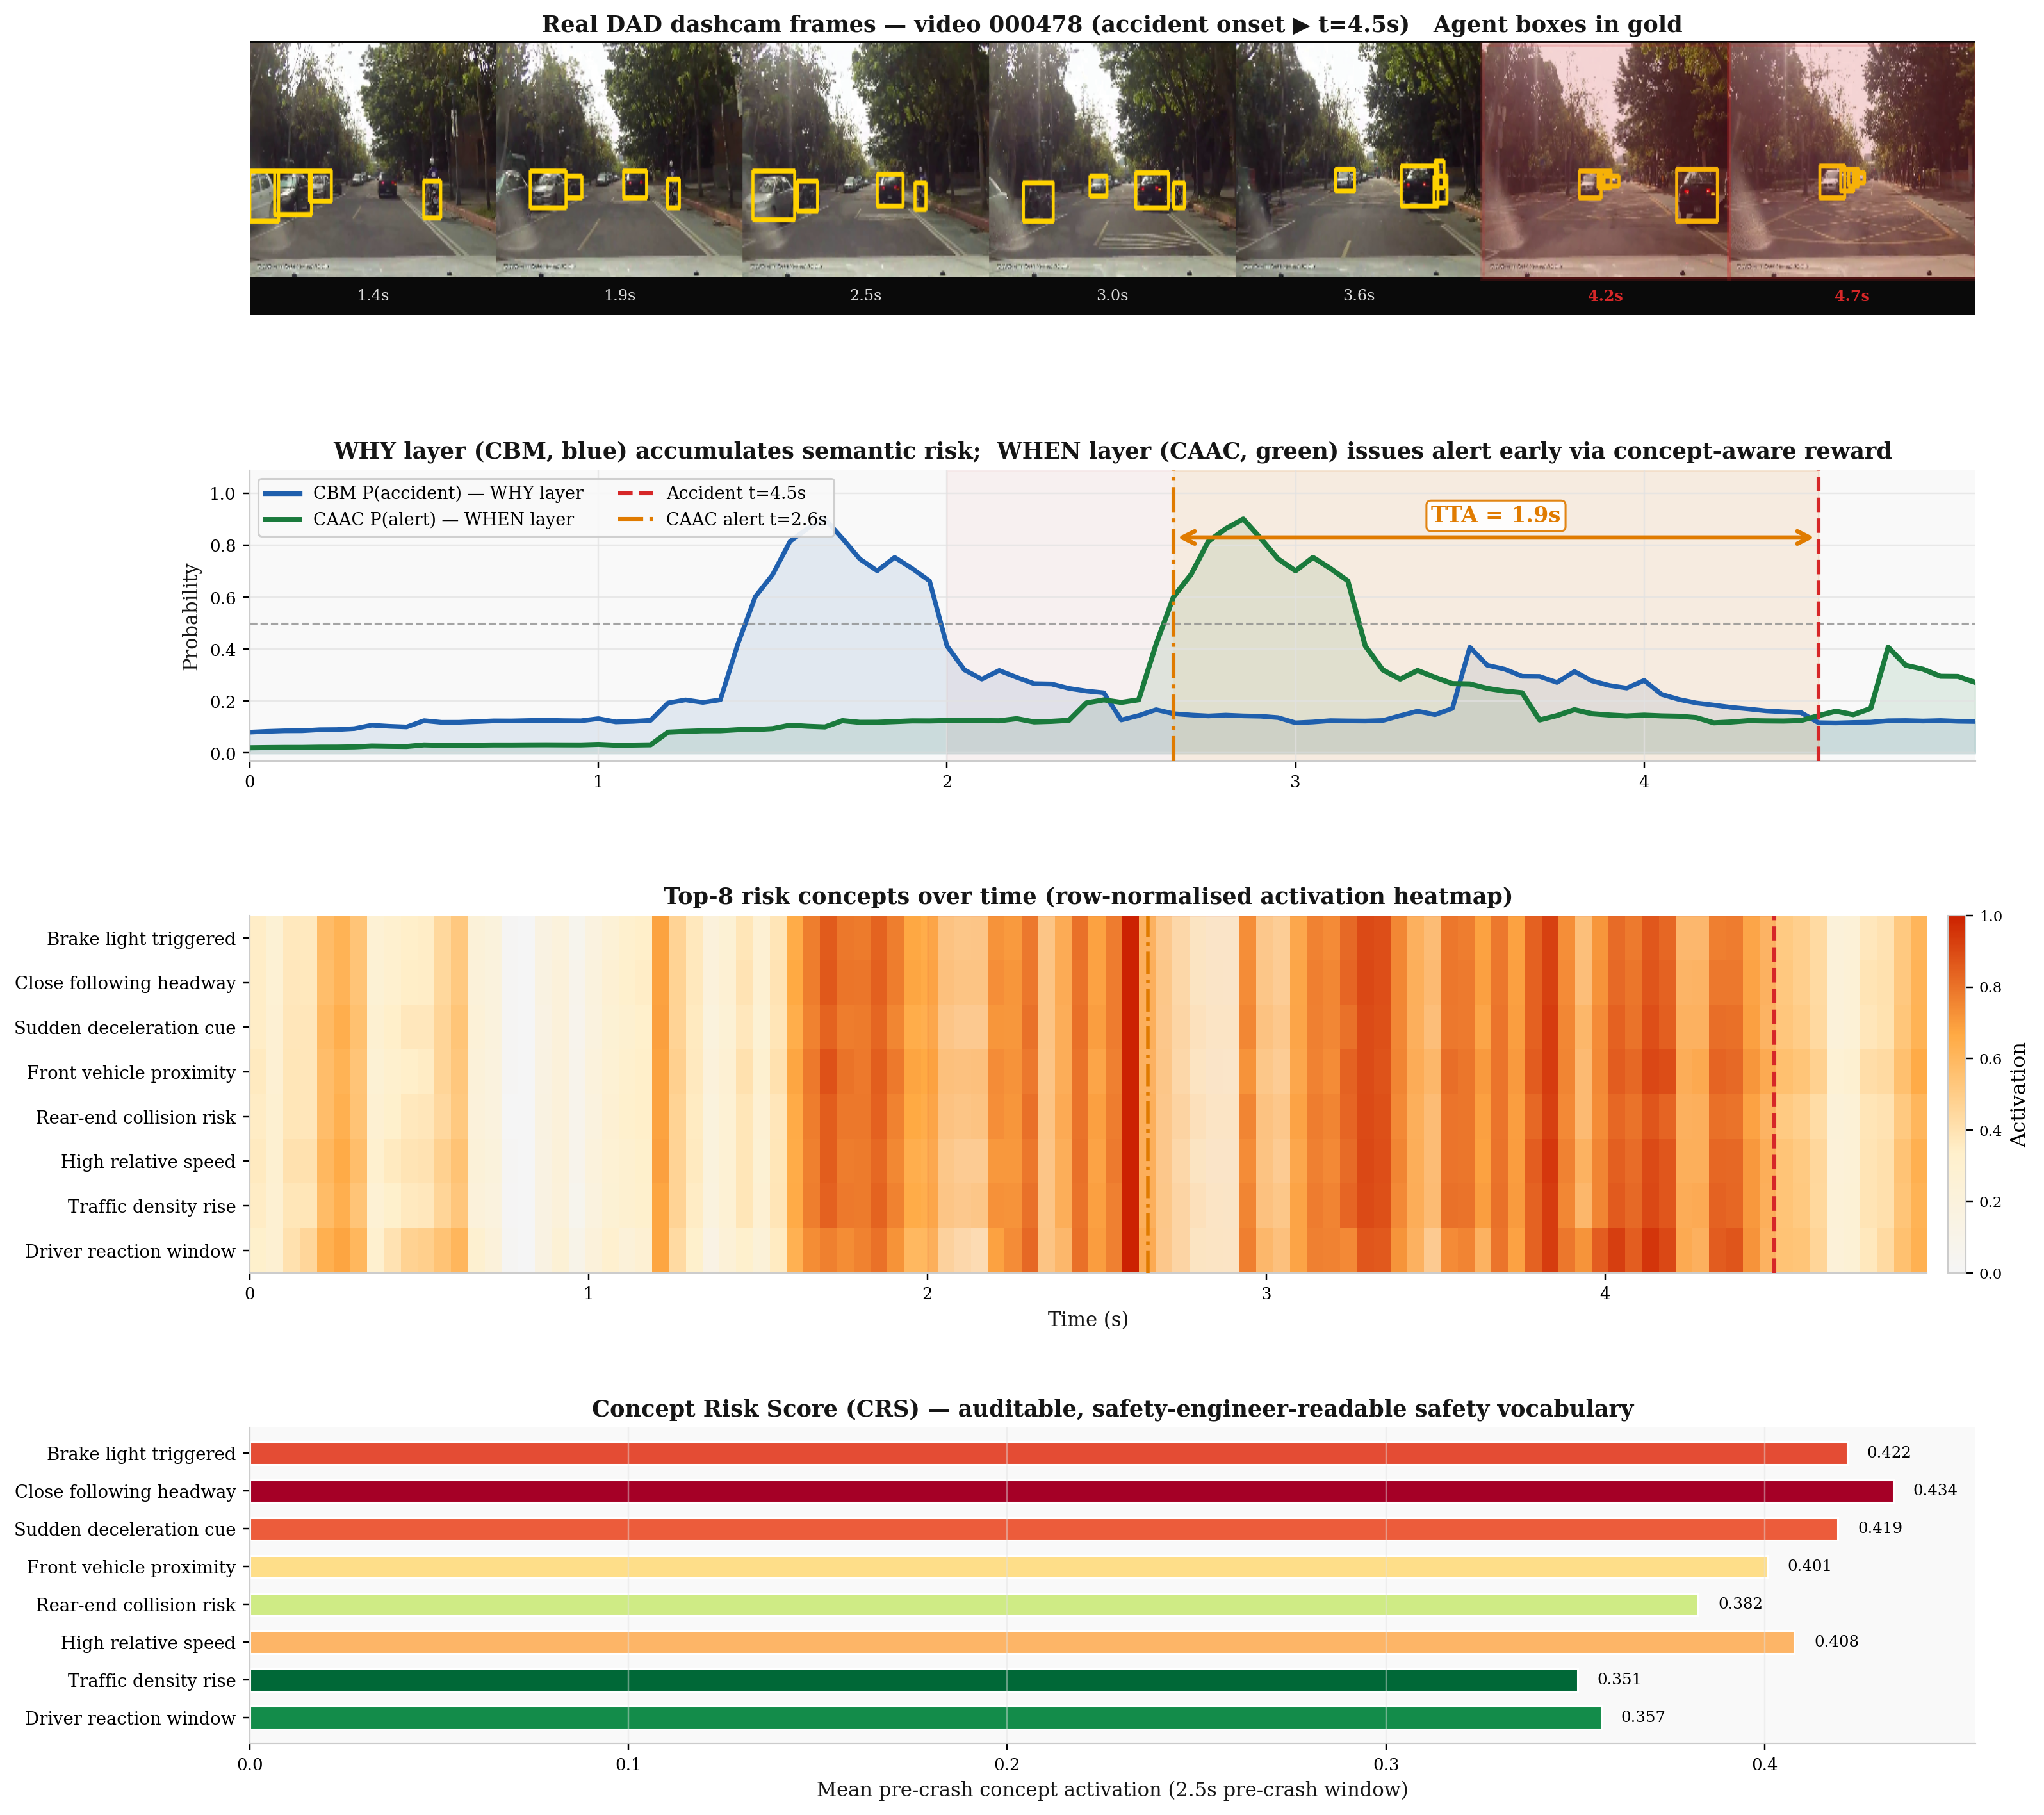
\includegraphics[width=0.98\textwidth]{../figures/insight_fig1_hero_dad_real.pdf}
  \caption{\textbf{A compact motivated example of the semantic interface.}
  One real crash sequence is read through named risk concepts before
  impact. The model does not expose only one final risk score; it exposes an
  inspectable semantic trajectory that can be inspected, compared, and audited
  as the scene evolves. The risk trajectory, concept activations, and alert
  marker are quantified in the headline, ontology, and timing-support evidence
  blocks rather than treated as a standalone case-study claim.}
  \label{fig:motivation}
\end{figure*}

\begin{figure*}[t]
  \centering
  \begin{subfigure}{0.495\textwidth}
    \centering
    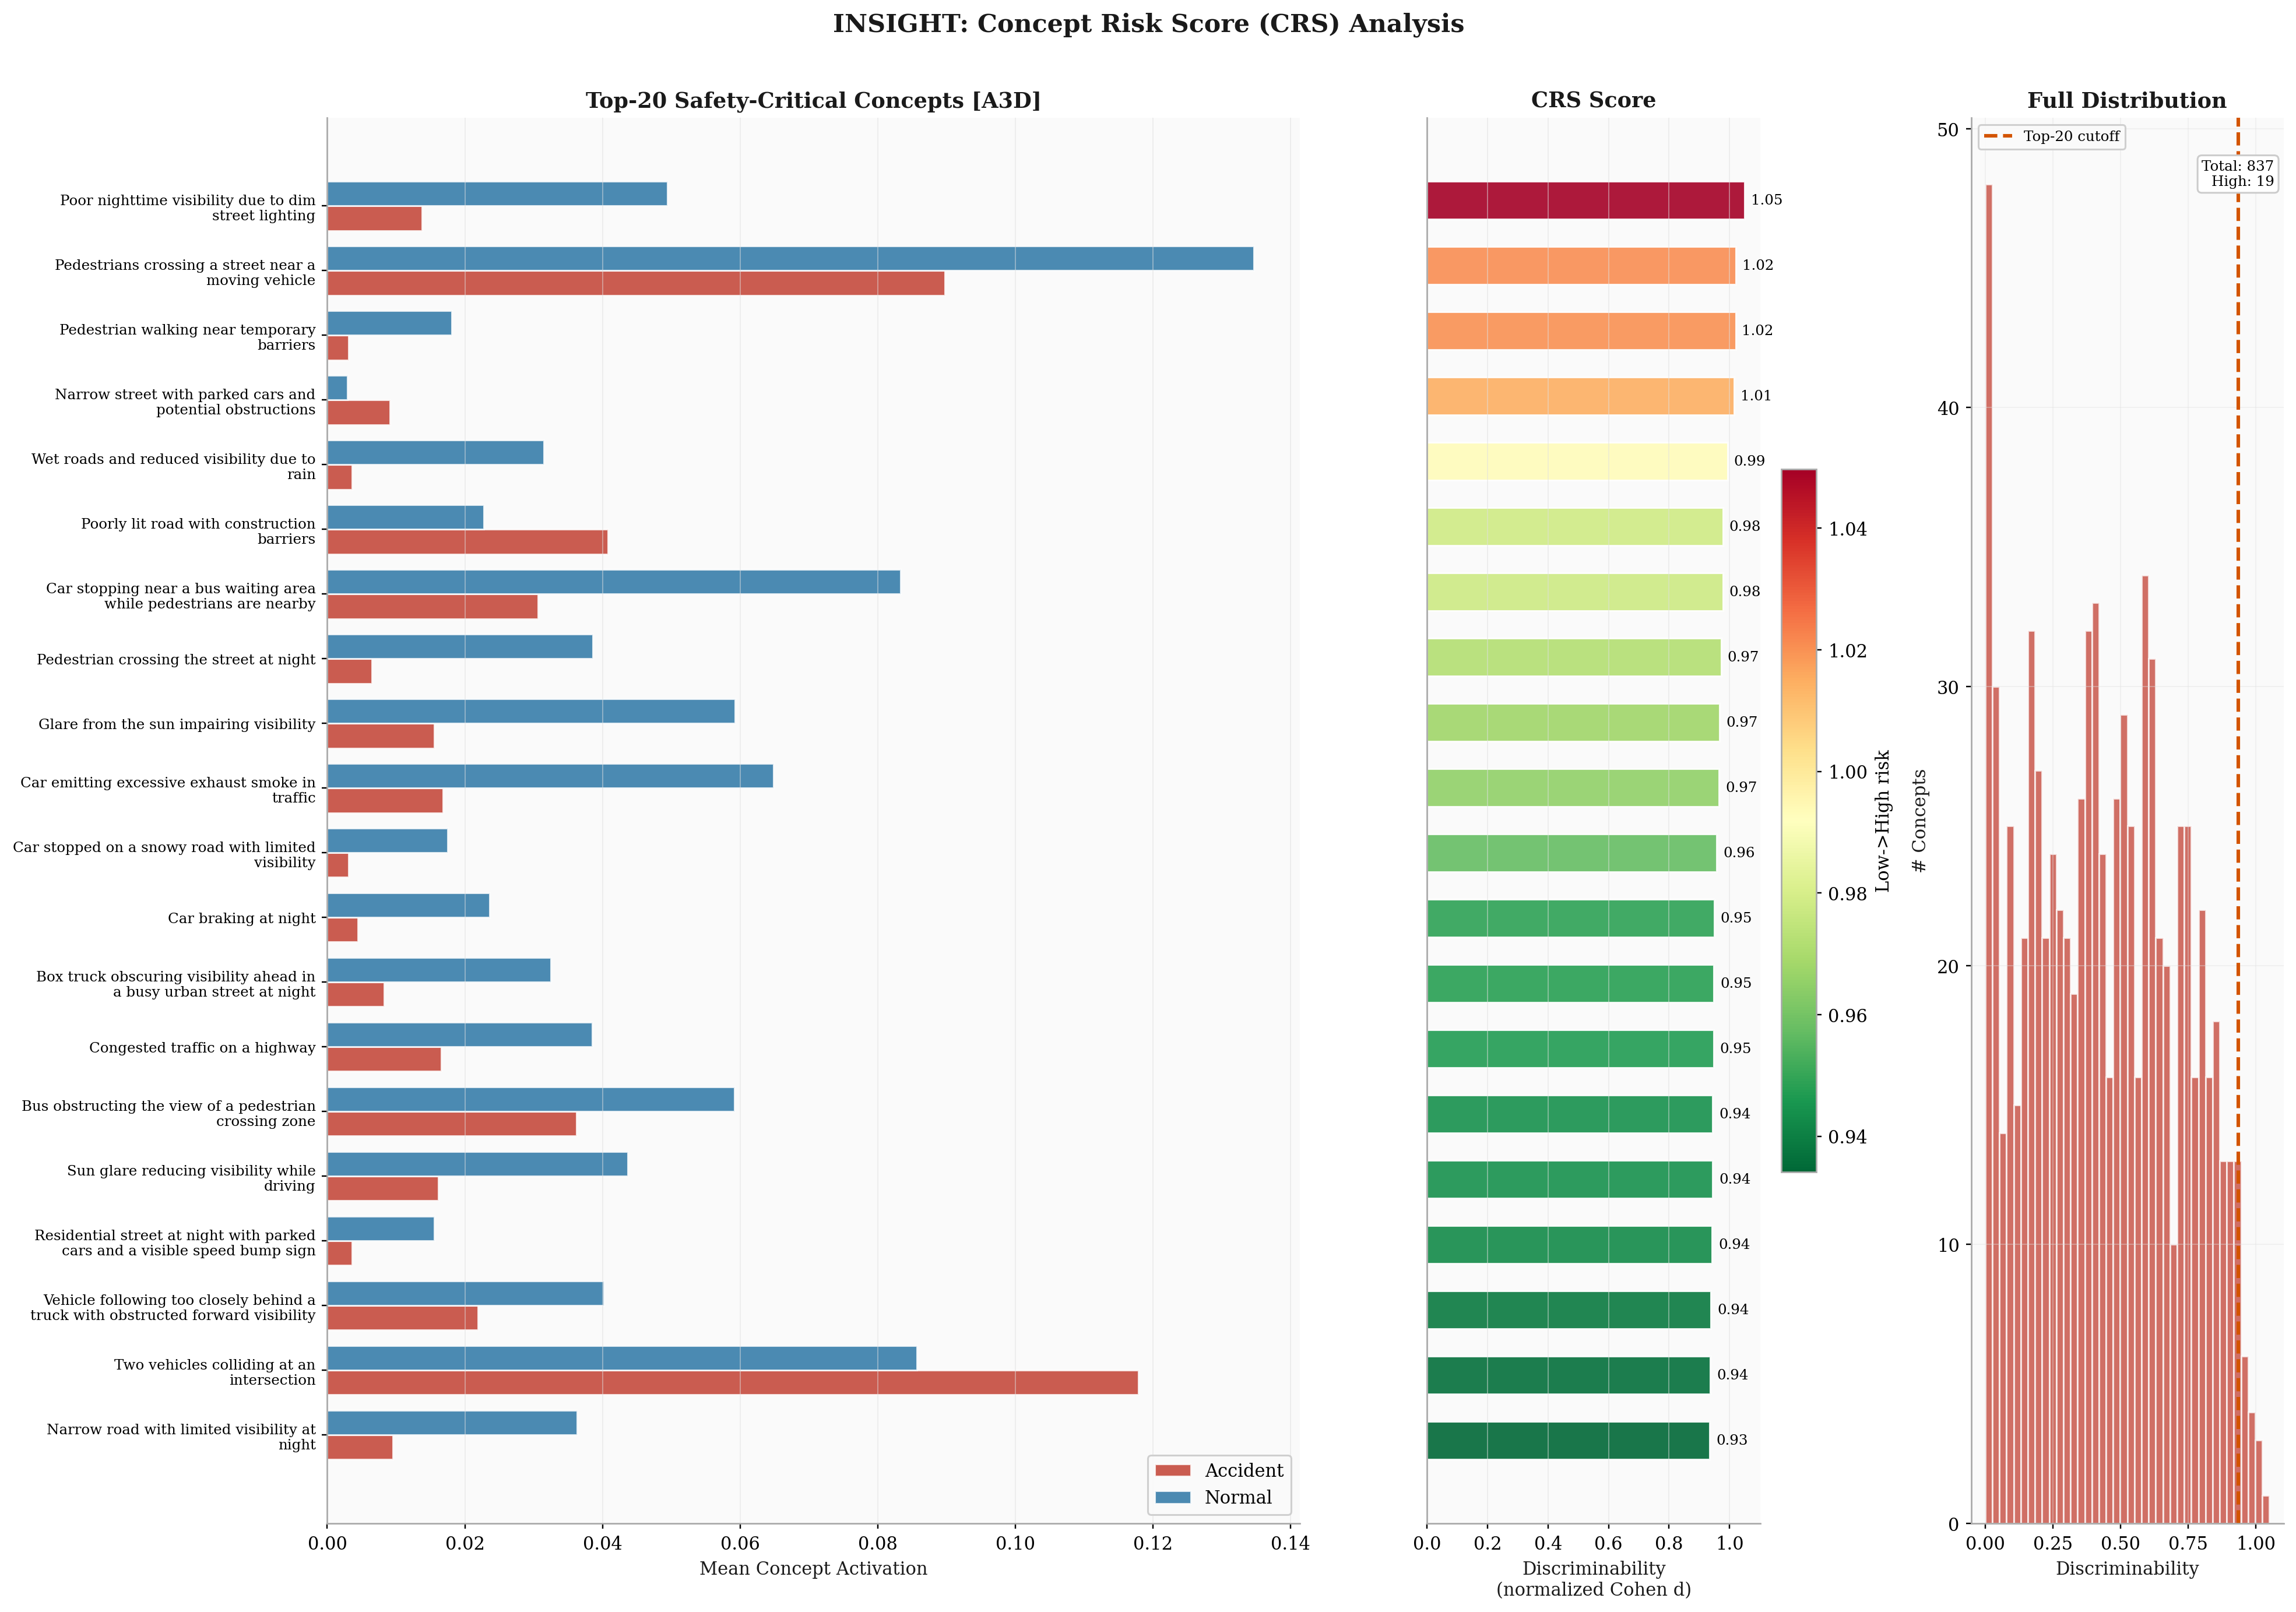
\includegraphics[width=\linewidth]{../figures/insight_fig3_crs_a3d.png}
    \caption{A3D CRS trace}
    \label{fig:vis_crs_a3d}
  \end{subfigure}
  \hfill
  \begin{subfigure}{0.495\textwidth}
    \centering
    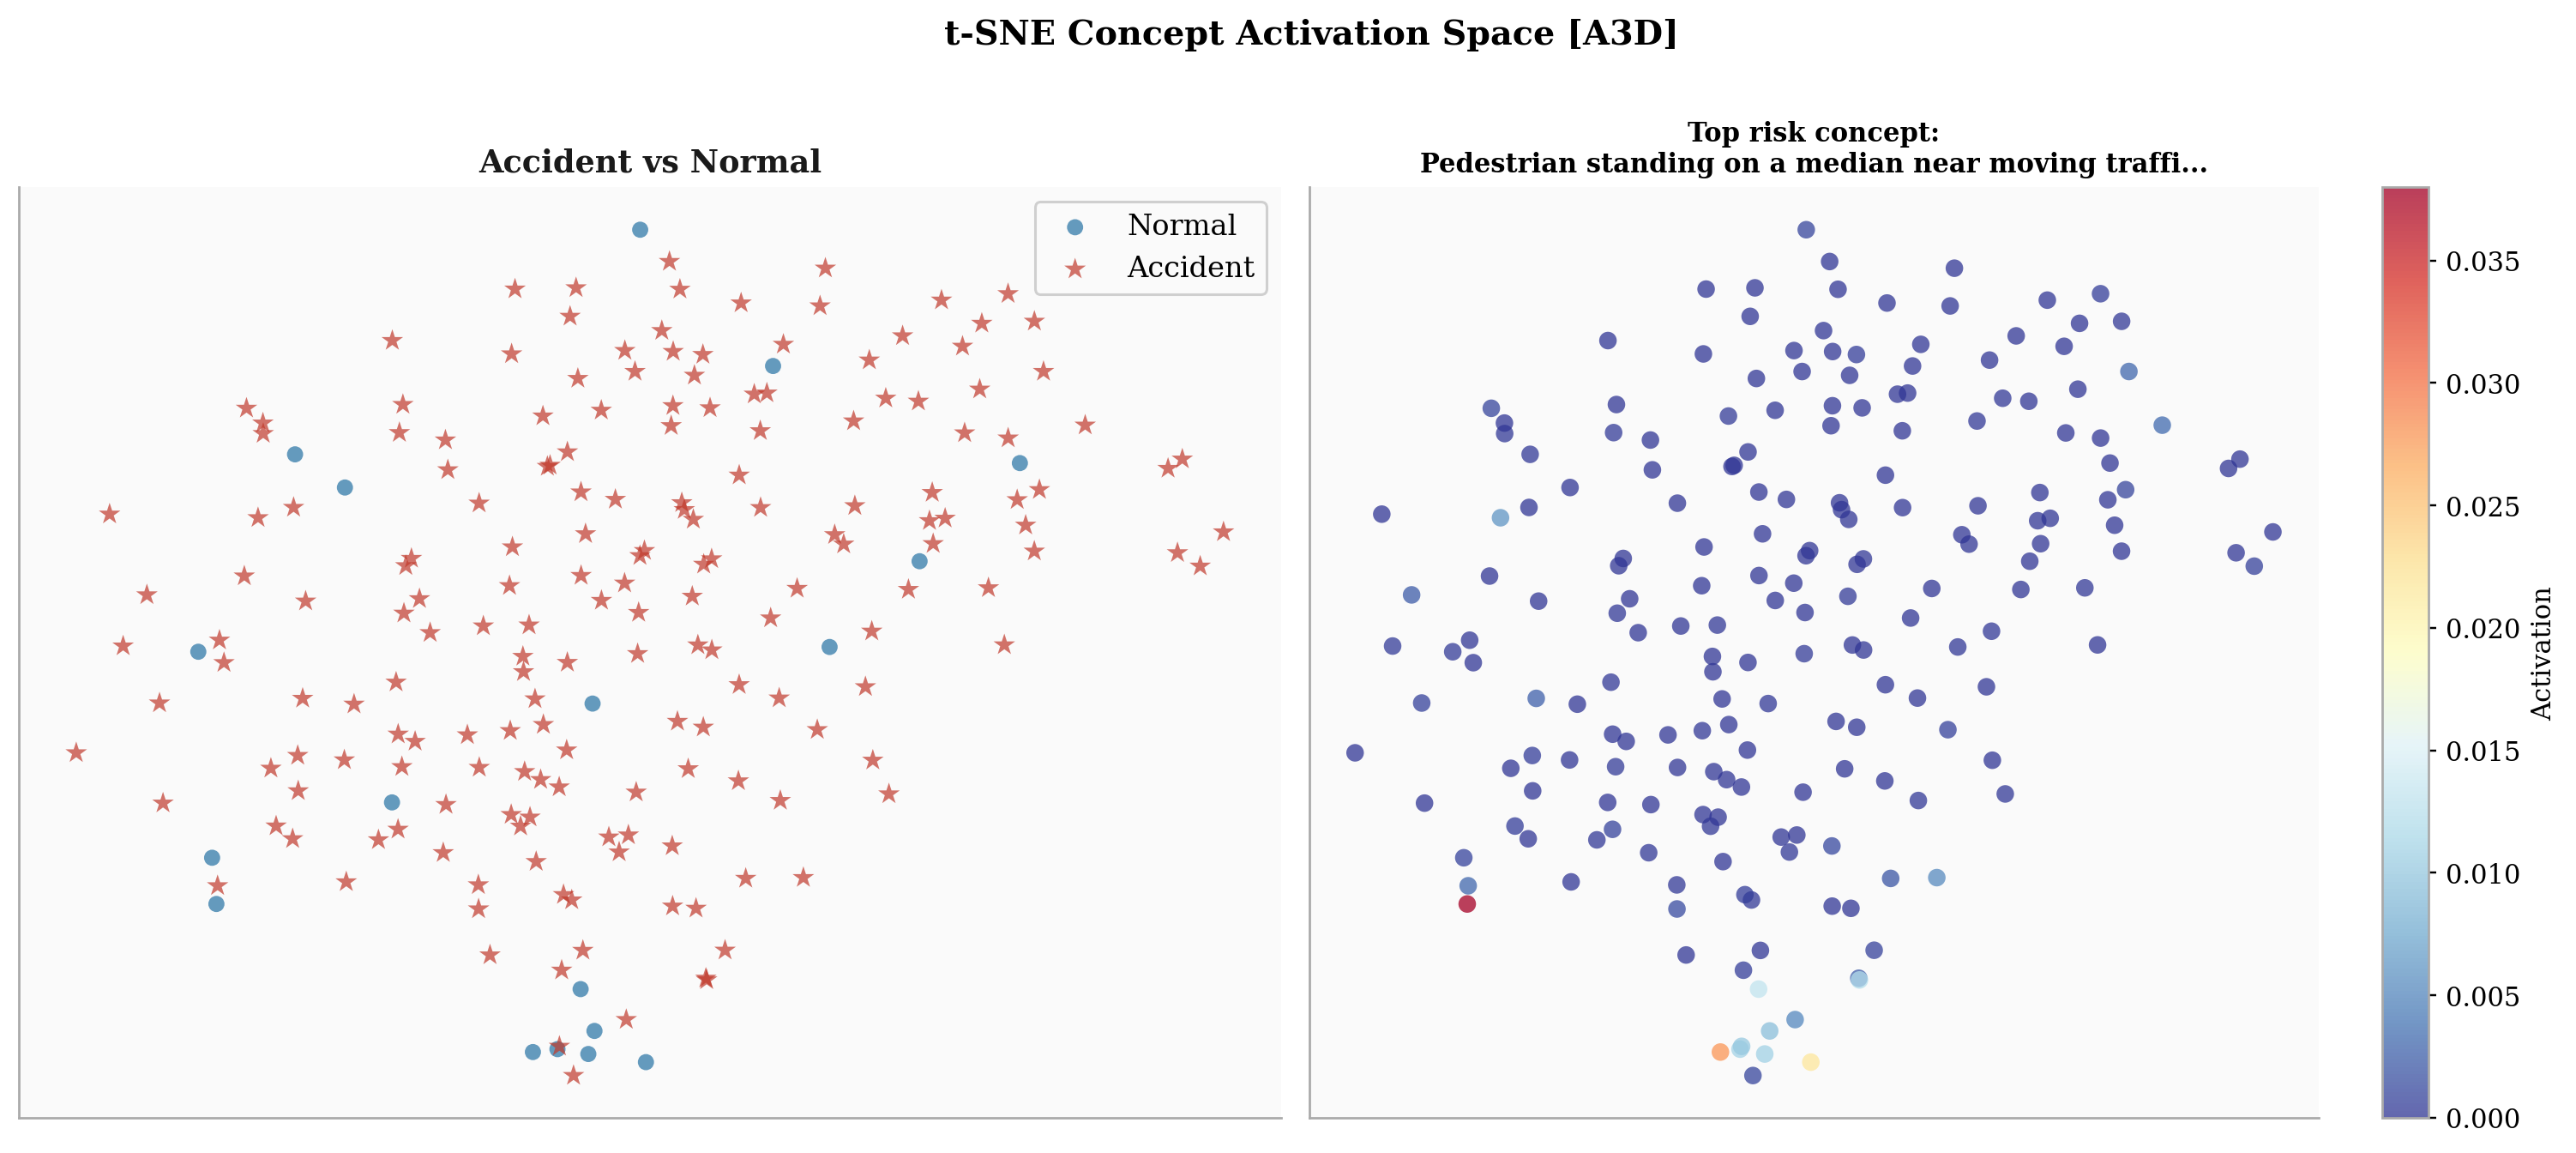
\includegraphics[width=\linewidth]{../figures/insight_fig4_tsne_a3d.png}
    \caption{A3D concept-space geometry}
    \label{fig:vis_tsne_a3d}
  \end{subfigure}
  \caption{\textbf{Interpretability bridge.}
  CRS and concept-space geometry provide a quick, intuition-first view of how the semantic interface behaves across pre-impact phases.
  }
  \label{fig:vis_bridge}
\end{figure*}

Figure~\ref{fig:motivation} and Figure~\ref{fig:vis_bridge} are intentionally paired with
Table~\ref{tab:a3d}, Table~\ref{tab:concept_sets}, and
Figure~\ref{fig:safety_utility}, Figure~\ref{fig:data_efficiency}, and
Figure~\ref{fig:intervention_gallery}:
the motivated example and bridge view show what the semantic interface looks like per case,
while the later headline/support blocks and the intervention gallery test whether
the same behavior survives quantitative, mechanistic, and cross-regime scrutiny.
The score trace and concept activations in Figure~\ref{fig:motivation} should
therefore be read as entry points to the quantitative ontology and timing
blocks, not as standalone evidence.


\paragraph{The missing object in accident anticipation: a semantic interface.}
The literature has made impressive progress on predictive quality.
Methods such as CRASH~\citep{liao2024crash}, CCAF-Net~\citep{liu2025ccaf}, and
LATTE~\citep{ZHANG2025103173} show that large-capacity models can deliver
strong AP and timing metrics. But from the perspective of interpretability and
scientific audit, a crucial object is still missing: an explicit semantic
interface between visual evidence and anticipation behavior. Without such an
interface, it is difficult to answer simple but important questions:
\emph{What risk concepts does the model actually rely on?}
\emph{How should those concepts be named, merged, or reviewed?}
\emph{Does changing the ontology change the predictive--timing trade-off?}

\paragraph{Why post-hoc explanation is not enough.}
Prior work offers only partial answers.
DRIVE~\citep{ref2} appends Grad-CAM after prediction;
W3AL~\citep{liao2024and} verbalizes accident location with an LLM;
other strong anticipation systems provide no intrinsic concept-level semantic
layer at all.
These approaches may help describe or localize a prediction, but they do not
turn the model's internal evidence into a stable, trainable, and auditable
representation that can be compared across runs or governed as a research
artifact. In a safety domain, that distinction matters: a system is easier to
audit and debug when its exposed semantics are part of the forward path, not an
after-the-fact visualization.

\paragraph{Scope we claim and do not claim.}
We make a focused claim: a language-grounded ontology is a governed research
variable, and that variable changes forecasting behavior in measurable ways under
matched training protocols.
We do not claim dataset-agnostic superiority, complete policy-level intervention control,
or that the same ontology choice is optimal across all driving distributions.
In this paper, CRASH materials are used as support-oriented stress and transfer
signals and are not pooled into the headline DAD/A3D claims.
This restraint is central to how we frame both our headline and support evidence.

\paragraph{Reading convention.}
We keep one compact convention throughout the paper: headline tables establish
the primary predictive position, controlled ontology comparisons test the
central semantic-interface claim, and stress analyses (including actor-policy
timing and CRASH transfer) are reported as bounded support evidence.

\paragraph{Our central insight.}
In accident anticipation, ontology construction should be treated as part of
the method rather than as hidden preprocessing.
A concept bottleneck is only as useful as the vocabulary it exposes. A generic
traffic word list is often too noisy; a fully manual ontology is hard to scale;
and an ungoverned pool of multimodal concept proposals is hard to defend as a
scientific interface. We therefore elevate concept construction itself to a
first-class modeling problem: sample risk-relevant frames, mine candidate risk
concepts, perform risk-first refinement, merge duplicates, balance semantic
families, and export a trainable ontology with explicit provenance. In the
language-interface framing of this paper, the key point is not merely that language is used
somewhere in the pipeline. It is that the language layer is governed:
canonical names, merge decisions, family structure, prompt policy, and light
review are all recorded as part of the research object.

\paragraph{\method{}: from risk ontology to trainable semantic interface.}
We propose \method{} (\textbf{In}terpretable \textbf{S}afety-\textbf{G}uided
accident anti\textbf{ci}pation via concep\textbf{t} bott\textbf{le}neck and
concept-aware actor-critic), but in this paper the center of gravity is
the \emph{language-grounded risk concept interface}. The model uses a
reproducible multimodal ontology pipeline to construct the semantic bottleneck,
then trains an interpretable anticipation system on top of that interface.
Concretely, the full framework contains
(i) a concept discovery and adjudication pipeline,
(ii) the \cbm{} semantic bottleneck,
(iii) the global \crs{} audit layer,
(iv)~\cgta{} for concept-linked temporal modeling,
(v)~\tsd{} for anticipatory representation learning, and
(vi) \caac{} as a downstream timing consumer of the concept state.
This design allows us to study not only model quality, but also how ontology
design changes the operating point of an interpretable anticipation system.
It also lets us separate three evidence questions cleanly: whether the
interface improves or preserves prediction quality, whether ontology choice
changes downstream behavior under matched training protocols, and whether the
release ontology's
canonical names and semantic families remain reviewable on the language side.

\paragraph{Contributions.}
\begin{itemize}[leftmargin=1.4em,topsep=2pt,itemsep=1pt]
  \item We argue that accident anticipation needs an auditable semantic interface, and that ontology construction should be treated as part of the method rather than hidden preprocessing.
  \item We introduce a reproducible multimodal risk-concept construction pipeline that mines, refines, merges, balances, and reviews risk concepts to produce a trainable ontology with explicit provenance, family structure, and canonical naming policy.
  \item We build \method{}, an interpretable anticipation framework that uses this ontology as a concept bottleneck and exposes auditable concept-level risk signals during prediction.
  \item We show, under matched training-protocol controls, that ontology choice changes the AP--mTTA operating point on both DAD and A3D, making the semantic interface itself an empirical variable rather than a cosmetic report.
  \item We pair predictive claims with language-side audits (500-frame pseudo-label and paraphrase stress), concept-level governance logs, and full review coverage for the released ontology. Under this protocol, \method{} reaches 93.40\% AP / 4.90s mTTA on A3D and 68.19\% AP on the canonical DAD line, while actor-policy timing is reported as scoped supporting evidence.
  \item We keep the central claim intentionally constrained: \method{} advances semantic-interface methodology and auditing, with the strongest current contribution in interpretability and controlled ontology science rather than policy-level causal intervention.
\end{itemize}
